\documentclass[seminar,english]{AIGpaper}
\usepackage{graphicx}					           % enhanced support for graphics
\usepackage{amsfonts}					           % math fonts
\usepackage{amssymb}					           % math symbols
\usepackage{amsmath}					           % overall enhancements to math environment
\usepackage{amsthm}                                % for theorems and other environments
\usepackage{url}                                   % for linking external urls
\usepackage[hidelinks]{hyperref}                   % for automatic hyperlinks
\usepackage{microtype}
\usepackage{fnpct}
\usepackage{caption}
\usepackage{subcaption}
\usepackage{float}

\DeclareCaptionLabelFormat{figsub}{(\thefigure#2)}
\captionsetup[subfigure]{labelformat=figsub}

\RedeclareSectionCommand[
  beforeskip=0pt
]{subparagraph}

\title{Seminar: Artificial Intelligence - Visual Computing\\3D Gaussian Splatting}
\author{Sebastian Frehmel}

\englishabstract{3D Gaussian Splatting (3DGS) denotes a seminal approach to 3D reconstruction and novel-view synthesis which was first published in 2023.
This paper introduces the underlying rationale and concepts of 3DGS for a Data and Computer Science audience outside of Computer Graphics. The original publication is analyzed in full detail with an emphasis on the constituent steps of the training procedure.}

\begin{document}
\maketitle

\section{Introduction to the Field of 3D Reconstruction}
3D Gaussian Splatting is a new technology in the field of 3D reconstruction which requires introducing certain basic terminology.

\textit{3D reconstruction} marks a field in Computer Graphics which allows creating 3D \textit{scenes} of different kinds from a given input like a set of images or frames of a video.
Once this 3D scene has been created, \textit{novel-view synthesis} refers to the process of gaining previously non-existing imagery from this 3D scene~\cite{liuSurvey3DReconstruction2025, tewariStateArtNeural2020}. However, both processes are commonly aggregated into the single term 3D reconstruction, a practice we do not adopt here.
Next, \textit{real-time novel-view synthesis} is the ability to synthesize new imagery at a rate of 24 to 30 frames per second (FPS) or more~\cite{heSurvey3DGaussian2026}, making it possible to smoothly explore a reconstructed scene comparable to commonly used non-reconstructed mesh-based scenes found e.g. in 3D gaming.

First efforts in this field date back to the 1990s with work on multi-view geometry~\cite{liuSurvey3DReconstruction2025} and remained a niche area of research due to lack of powerful models until the general emergence of neural networks in the late 2010s. 
Neural networks for the first time allowed creating 3D scenes with realistic image quality using the radiance field approach.
An \textit{implicit radiance field}~\cite{hubertEditingImplicitExplicit2025a} is based on the mathematical concept of the five-dimensional plenoptic function $L: x, y, z, \delta, \phi \rightarrow c, \alpha$ which expresses a scene by continuously mapping any given point $(x, y, z)$ in space and a set of viewing angles $\delta$ and $\phi$ (pitch and yaw) to a color $c$ and an opacity $\alpha$ at that point.
\begingroup
\clubpenalty=0
\widowpenalty=0
\textit{Explicit radiance fields} restrict the plenoptic function to a finite set of points, for example using a rigid 3D \textit{voxel} grid.
\par
\endgroup

One well-known implementation of radiance fields are \textit{Neural Radiance Fields} (NeRFs) introduced by Mildenhall et al. in 2020~\cite{mildenhallNeRFRepresentingScenes2020}. NeRFs take a set of input images and use a neural network to learn an implicit radiance field representation of the resulting scene, which means the full scene is encoded in the neural network's weights.
In order to perform novel-view synthesis for a NeRF, a technique called \textit{volumetric ray marching} is employed. 
For every pixel in the novel view the NeRF algorithm transmits a ray through the implicit radiance field resulting in a very high number of queries to the neural network for each (discretized) point along the path of the ray before adding up all predicted RGB and opacity values to form the final color value of each pixel~\cite{mildenhallNeRFRepresentingScenes2020}.
For more information on NeRFs refer to the previous paper in this seminar.

The other aspect which is important to know is the concept of \textit{splatting}. First introduced in 1991 by Westover~\cite{Westover1991SplattingAP} and refined later in the early 2000s by a group around Zwicker~\cite{zwickerEWAVolumeSplatting2001, zwickerSurfaceSplatting2001}, it takes the reverse approach to ray marching by projecting all elements in the 3D scene onto the view plane towards the camera, a process which colloquially can be called ``splatting'' or ``squashing''. 
It was also Zwicker et al. in the same publications who introduced \textit{3D Gaussians} as a data structure to simplify and extend splatting.

Lastly, there are important basic concepts in Computer Graphics that need explaining especially in the context of splatting, starting with \textit{world space}, \textit{view space}, and \textit{image space}. The first describing the space in which the 3D scene is built; the second describing the same space shifted with the camera at the origin; and the third describing the space after \textit{camera projection}.
Then there is the near plane, also called the \textit{view plane} or projection plane and the \textit{far plane} as well as the \textit{camera pose} or position. The camera pose and its \textit{field of view} (FOV) decide which elements of the scene between the view plane and the far plane are to be included in the projection onto the view plane.
This setup is known as the ``pyramid of vision'' or \textit{view frustum} as it takes the shape of a frustum, see Figure~\ref{fig:view_frustum} on page~\pageref{fig:view_frustum}. \textit{Frustum culling} removes all elements outside the view frustum. For more general aspects of computer graphics see~\cite{marschnerFundamentalsComputerGraphics2021}.

Training NeRFs to reach photorealistic scene quality can take several days on professional high-end GPU hardware, as is the case with e.g. Mip-NeRF, a NeRF-based system reaching highest PSNR\footnote{Peak signal-to-noise ratio, used to evaluate quality of reconstruction as perceived by a human} scores among NeRFs.
Also, during novel-view synthesis, ray marching is very time-consuming as the neural network has to be queried very often and the algorithm cannot determine if a ray has reached sufficient opacity. In other words, a ray always has to travel through the entire implicit radiance field representation of the neural network.
This has led to some implementations of NeRFs switching to explicit radiance field representations and losing the neural network for novel-view synthesis allthogether (e.g. ''Plenoxels'') which comes at the inherent cost of reduced image quality due to fewer and less precise points in the radiance field.
These approaches do allow training times of 20-30 minutes and make it possible to come close to real-time novel-view synthesis reaching around 10-15 FPS at 1080p resolution. 
Other downsides of NeRFs include possibly having to sample empty space along the ray, as well as not being able to easily edit or amend a reconstructed scene as these details are all hidden in the weights of the neural network (''black box''). 
So either NeRFs allow state-of-the-art reconstruction quality at the cost of long training and synthesis times while only being able to synthesize single images or they have to reduce reconstruction quality to be able to reduce training times and come somewhat close to real-time novel-view synthesis.

To overcome the mentioned drawbacks of NeRFs, Kerbl et al \cite{kerbl3DGaussianSplatting2023} at INRIA in France introduced 3D Gaussian Splatting (3DGS) in late 2023, which makes it a very recent technology. Yet, their paper has had fundamental impact in the field of 3D reconstruction and elsewhere standing at nearly 11.000 citations \cite{researchGateKerbl} in less than three years. 

Kerbl et al managed to to combine previously existing concepts of splatting and 3D Gaussians to create a learnable explicit radiance field representation. Key to this approach is the fact that 3D Gaussians are differentiable and can be used in standard backpropagation procedures using gradient descent. Most importantly, this means that 3DGS does not use neural networks at all.

Using 3D Gaussians, a concept which we will explain in the next chapter, as the base primitive for 3D reconstruction furthermore allows for arbitrary precision and does not suffer from issues explicit radiance field representation had when used in NeRFs. Using 3D Gaussians also enables direct editability of the scene, such as additions or lighting changes making it much more accessible and subsequently usable for downstream applications.

The other important cornerstone of Kerbl et al's publication was the major engineering achievement of mapping this new idea perfectly onto modern GPU hardware for both, 3D reconstruction and novel-view synthesis, resulting in speed-ups that had not been seen before in this field. The centerpiece here is the tile-based rasterizer, which we will also cover in-depth in chapter \ref{ch:rasterizer}.

This way they created the first explicit, differentiable, unstructured and primitive-based radiance field architecture finally allowing real-time novel-view synthesis at 1080p resolution while matching or even improving scene quality in comparison to state-of-the-art NeRF architectures.

This paper will explain the underlying mechanics and concepts of 3DGS in detail. The original paper by Kerbl et al appears very packed leaving out many details, moving them to a project website and a GitHub repository.
Even many of the subsequent papers do not discuss the algorithmic approaches - which in fact have only been minorly altered since inception - so that this seminar paper takes a deep dive for an audience outside of computer graphics which is currently not being taught at Fernuniversität Hagen while emphasizing the machine learning/AI aspects.
We will begin with 3D Gaussians as the fundamental data structure and continue with the training and novel-view synthesis processes following the original paper closely before showing selected improvements to the algorithm and giving insights into 3DGS applications with a focus on dynamic scene reconstruction.

Analyzing the original authors' \cite{kerbl3DGaussianSplatting2023} repository \cite{kerblRepo} or consulting survey papers like \cite{bagdasarian3DGSzipSurvey3D2025} indicates that a 3D Gaussian is a data structure consisting of 14 to 59 attributes:

\begin{itemize}
    \item Position $\mu$: three-dimensional coordinates in worldspace for the origin of the 3D Gaussian. (3 attributes)
    \item Opacity $o$: the peak opacity at point $\mu$. Can be any number but is passed through a sigmoid function to bound it to $(0,1)$. (1 attribute)
    \item Covariance matrix $\Sigma$: A $3\times 3$ matrix determining 3D shape and rotation of the 3D Gaussian, but decomposed into three scaling values and four rotational values (''quaternions''). Decomposing the covariance matrix is pivotal for the backpropagation process, see chapter \ref{ch:matrix_decomp}. (7 attributes)
    \item Spherical harmonics coefficients: model view-dependent colors and specular reflections. Spherical harmonics come in four degrees \cite{plenoctrees}. SH0 is a simple RGB value denoting a solid color of the 3D Gaussian that is not dependent on viewing angles. Degrees SH1 to SH3 contribute 15 attributes each adding more and more to realism. SH3 is recommended for 3DGS  \cite{kerbl3DGaussianSplatting2023}. For the remainder of this paper we will disregard spherical harmonics and their complexity as the processes for training and novel-view synthesis can be explained without any notion of color. (3-48 attributes)
\end{itemize}
The reason the 3D Gaussian is called \textit{Gaussian} lies in its opacity distribution $\alpha$ which is modelled after the dimension-agnostic form of the normal distribution \cite{zwickerSurfaceSplatting2001}: $$ \alpha(p) = o \times \exp\left(-\frac{1}{2}(p - \mu)^T \Sigma^{-1}(p - \mu)\right) $$ with $p$ being any point in worldspace and $\Sigma^{-1}$ the inverse of the covariance matrix.
In other words we multiply the peak opacity value with a probability from the three-dimensional normal distribution shaped by $\Sigma$. This way, a 3D Gaussian becomes rapidly more transparent toward its edges. Mathematically each 3D Gaussian reaches into infinity with values asymptotically near 0 the farther from the center the opacity is being calculated. 
To remedy this effect, 3DGS enforces a hard 3-Sigma boundary meaning that everything outside of three standard deviations from $\mu$ is being culled, establishing an ellipsoid bounding shape which captures 99.7\% of the 3D Gaussian.

The shape a 3D Gaussian takes is therefore only defined by the density of its opacity distribution or as it is usually visualized, by its ellipsoid bounding shape.

\subsection{3D Gaussian Covariance Matrix Decomposition}
\label{ch:matrix_decomp}
For the entire learning process to work with backpropagation and gradient descent, a 3D Gaussian has to be differentiable. The original inception of a 3D Gaussian by Zwicker et al \cite{zwickerSurfaceSplatting2001} did not account for differentiability (or spherical harmonics for that matter), they were focussed on elaborating on the concept of splatting. 

During backpropagation the algorithm would have to come up with new, better values
\newpage %TODO
for the covariance matrix $\Sigma$ toward the direction gradient descent is pointing. However, in order to make sense geometrically, a covariance matrix in this case has to be positive semi-definite which means the determinant has to be $>=0$. 
As running a loop during backpropagation to find new valid values for the entire covariance matrix until the whole matrix is positive semi-definite again while still satisfying gradient descent would be far too costly, Kerbl et al \cite{kerbl3DGaussianSplatting2023} proposed a clever decomposition of the convariance matrix.

$\Sigma$ can be decomposed into a $3\times 3$ scaling matrix $S$ and a $3\times 3$ rotational matrix $R$: $\Sigma = RSS^TR^T$ which is itself just an instance of the default eigendecomposition $\Sigma = Q\Delta Q^T$ with eigenvectors $Q$ (rotations) and a diagonal matrix of eigenvalues $\Delta$ (scaling). Lastly, since $S$ is a diagonal matrix, $SS^T=S^2=\Delta$.

The scaling matrix can now be decomposed into three scaling values $[s_1, s_2, s_3]$ which are the roots of the eigenvalues of $\Sigma$. Also, the rotational matrix can be further decomposed into four values $[w, x, y, z]$ called \textit{quaternions}, a concept used in aviation, in the following way \cite{Shoemake1985AnimatingRW}:$$R = \begin{bmatrix} 1 - 2(y^2 + z^2) & 2(xy - wz) & 2(xz + wy) \\ 2(xy + wz) & 1 - 2(x^2 + z^2) & 2(yz - wx) \\ 2(xz - wy) & 2(yz + wx) & 1 - 2(x^2 + y^2) \end{bmatrix}$$

With the covariance matrix fully decomposed into two smaller components, 3DGS only ever stores these seven values for each 3D Gaussian and treats each component separately in the backpropagation process. A new covariance matrix can be constructed from both components which is guaranteed to be positive semi-definite and thus geometrically valid since an eigendecomposition is always positive semi-definite \cite{riedel2025mathematische}.


Training a 3DGS scene starts with a point cloud which we take as the initial positions for 3D Gaussians. After that forward and backpropagation steps similar to those in neural networks \cite{thimm2025ML} alternate, modifying opacity, position, shape and color of each 3D Gaussian in the scene.
Pivotal for training quality is so-called \textit{Adaptive Density Control} which periodically steps in after backpropagation, further modifying 3D Gaussians.

In this chapter we will closely follow Kerbl et al \cite{kerbl3DGaussianSplatting2023} and their GitHub repository \cite{kerblRepo}. The entire training procedure is based on neural rendering concepts introduced by Yifan et al \cite{yifanDifferentiableSurfaceSplatting2019} and ''Pulsar'' by Lassner and Zollhöfer \cite{lassnerPulsarEfficientSpherebased2021} which can be seen as the direct predecessor of the rendering pipeline used for 3DGS. However, there are only very few papers that directly disect the pipeline math (like \cite{huang2DGaussianSplatting2024} or \cite{yuMipSplattingAliasFree3D2024} when improving the algorithm) as most papers use 3DGS for various applications. This is why much content in this chapter originates from in-depth websites like the formidable MrNeRF Github repository \cite{githubMrNerf} which provides further links.

\subsection{Point Cloud Initialization}
Initialization in 3D reconstruction is a crucial step as the positions of the initial points or primitives decide how well the algorithm can reconstruct a scene.

In order for the 3DGS learning algorithm to work, 3DGS needs initial geometry which is commonly a set of initial 3D Gaussians. This initial set is derived from input imagery such as photos or frames of a video. If the camera poses of this input imagery are not given directly, which is usually the case, the camera poses have be derived dynamically from the imagery.
A camera pose is designated by a $4\times 4$ \textit{extrinsic matrix} $W$ \cite{marschnerFundamentalsComputerGraphics2021} consisting of the $3\times 3$ rotational matrix $R$ (or $W_{rot}$) which contains the orientation of a camera in 3D space, a $3\times 1$ translation vector $t$ denoting the position of the camera in worldspace and a padding row to make $W$ square: $$W=\begin{bmatrix} R_{11} & R_{12} & R_{13} & t_x \\ R_{21} & R_{22} & R_{23} & t_y \\ R_{31} & R_{32} & R_{33} & t_z \\ 0 & 0 & 0 & 1 \end{bmatrix}$$
This matrix will become important later during forward and backpropagation steps.

The other component of a camera pose is the \textit{intrinsic matrix} which holds parameters of the camera lens like the focal length.

The defacto standard concept in 3D imaging to derive these two matrices for each input image is called \textit{Structure from Motion} (SfM) \cite{ullmanInterpretationStructureMotion1979} offered through a software called \textit{COLMAP}. SfM solves a large geometric optimization problem which finds common keypoints across all input imagery and uses them to provide highly accurate camera poses and a 3D point cloud of the scene. 

3DGS as originally conceived by Kerbl et al uses these points as the origins for the initial 3D Gaussians which are being initialized as perfect spheres with radii deduced from the three neighboring spheres with an opacity of around $0.1$.
The initial color can be any RGB value.

Consequently, having to derive camera poses for initialization first adds significantly to the entire training process which is why other, faster COLMAP-free methods have been proposed, see chapter \ref{ch:improvements}. Also, the authors mention that using random initialization of all 3D Gaussians yields good quality results even though training times are longer.

Finally, the natural logarithm is applied to all initial attribute values of a 3D Gaussian to be compatible with the initial forward pass.


\subsection{Forward Pass}
\label{ch:forwardpass}
At the beginning of each forward pass the algorithm selects an input image and its camera matrices (see chapter \ref{ch:matrix_decomp}) at random. Each forward pass and subsequent backward pass will only deal with one and the same input image.

In principle the forward pass is performing the splatting operation of all 3D Gaussians in the scene to produce a new image. This image will then be evaluated against the original input image using a loss function which the backpropagation step takes as input.

\subsubsection{Phase 1}

\subsubsection{Phase 2}

\subsubsection{Phase 3}

\subsubsection{Phase 4}

\subsubsection{Phase 5}
\subsection{Backpropagation}
\label{ch:backprop}
\subsubsection{Phase 1}

\subsubsection{Phase 2}

\subsubsection{Phase 3}

\subsubsection{Phase 4}

\subsubsection{Phase 5}

\subsubsection{Adaptive Density Control}
\label{ch:density_control}
Test

\vspace{-5pt}
\section{Novel-View Synthesis}
Once the scene has been trained as per the previous chapter, we can use the camera matrices of a novel view and execute the existing forward pass to render a new image.

\vspace{-5pt}
\section{Conclusion \& Outlook}
Kerbl et al. did not invent 3D Gaussians, nor splatting, nor 3D covariance matrix decomposition, nor spherical harmonics, nor neural or differential rendering, nor alpha compositing, nor explicit radiance fields, nor many other technologies. They experienced the progress and the remaining limitations that NeRFs brought yet whitnessed even explicit radiance field solutions for NeRFs not reaching real-time novel-view synthesis.

However, they resurrected 3D Gaussian Splatting from the depths of academia and repurposed it for the current age, took all of these existing components and experiences and realized that decomposing a 3D covariance matrix into scale and quaternions would always yield a geometrically valid covariance matrix and that passing these two components separately into backpropagation would elegantly solve previous issues.

The other half of what they contributed with 3DGS was how elegantly their algorithm fit onto the hardware, especially the ultra-fast Radix Sort and tile-based rasterizer.

3DGS has made easy 3D reconstruction feasible leading to many adaptions in real-world scenarios and ongoing massive research in the field, e.g. exceeding \textit{1000} FPS in special types of novel-view synthesis \cite{NEURIPS2025_6c39d1a7} or advances in SLAM in robotics \cite{keethaSplaTAMSplatTrack2024}, and many more.
\newpage

\appendix

\section{Figures}

\begin{figure}[H]
    \centering
    \begin{subfigure}{0.45\textwidth}
        \centering
        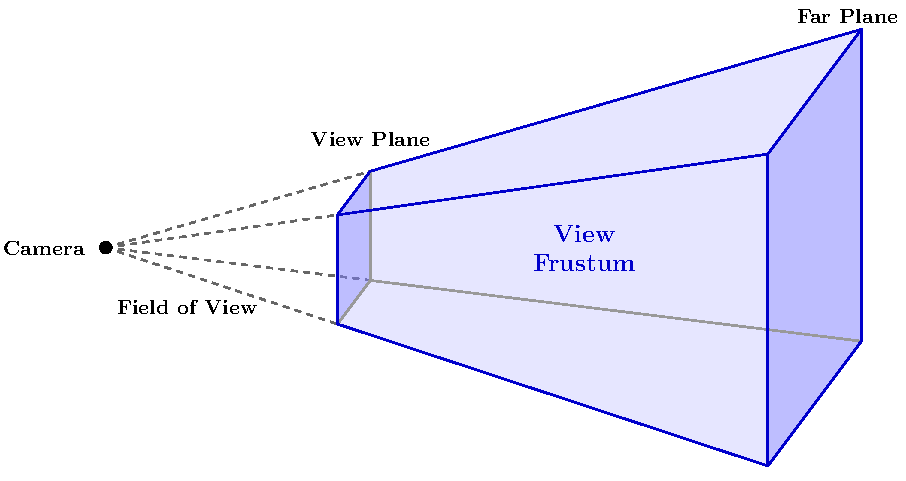
\includegraphics[width=\textwidth]{figures/view_frustum.pdf}
        \caption{View Frustum}
        \label{fig:view_frustum}
    \end{subfigure}
    \hfill
    \begin{subfigure}{0.45\textwidth}
        \centering
        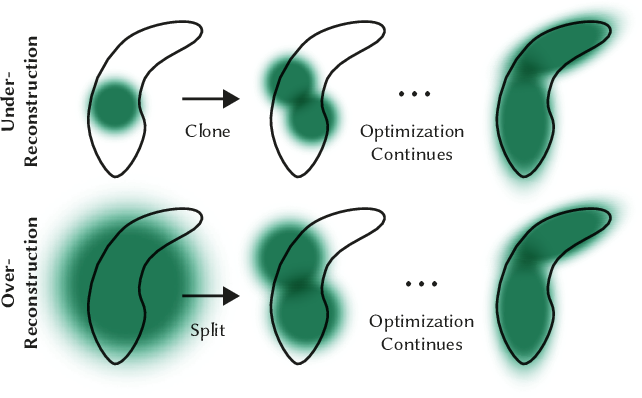
\includegraphics[scale=0.26]{figures/6-Figure4-1.png}
        \caption{Adaptive Density Control (from \cite{kerbl3DGaussianSplatting2023})}
        \label{fig:adc}
    \end{subfigure}
\end{figure}

\bibliographystyle{plain}
\bibliography{references}

\makestatement{1}
\end{document}